\iffalse
\let\negmedspace\undefined
\let\negthickspace\undefined
\documentclass[journal,12pt,twocolumn]{IEEEtran}
\usepackage{cite}
\usepackage{amsmath,amssymb,amsfonts,amsthm}
\usepackage{algorithmic}
\usepackage{graphicx}
\usepackage{textcomp}
\usepackage{xcolor}
\usepackage{txfonts}
\usepackage{listings}
\usepackage{enumitem}
\usepackage{mathtools}
\usepackage{gensymb}
\usepackage{comment}
\usepackage[breaklinks=true]{hyperref}
\usepackage{tkz-euclide} 
\usepackage{listings}
\usepackage{gvv}                            \usepackage{tikz}
\usepackage{circuitikz}
\def\inputGnumericTable{}                                
\usepackage[latin1]{inputenc}                            
\usepackage{color}                                       
\usepackage{array}                                       
\usepackage{longtable}                                   
\usepackage{calc}                              
\usepackage{tikz}
\usepackage{multirow}                                    
\usepackage{hhline}                                      
\usepackage{ifthen}                            
\usepackage{caption}
\usepackage{lscape}
\usepackage{amsmath}
\newtheorem{theorem}{Theorem}[section]
\newtheorem{problem}{Problem}
\newtheorem{proposition}{Proposition}[section]
\newtheorem{lemma}{Lemma}[section]
\newtheorem{corollary}[theorem]{Corollary}
\newtheorem{example}{Example}[section]
\newtheorem{definition}[problem]{Definition}
\newcommand{\BEQA}{\begin{eqnarray}}
\newcommand{\EEQA}{\end{eqnarray}}
\newcommand{\define}{\stackrel{\triangle}{=}}
\theoremstyle{remark}
\newtheorem{rem}{Remark}

\begin{document}

\bibliographystyle{IEEEtran}
\vspace{3cm}

\title{GATE 2021 NM Q24}
\author{EE23BTECH11009 - AROSHISH PRADHAN$^{*}$% <-this % stops a space
}
\maketitle
\newpage
\bigskip
\textbf{Question:} The sum of the infinite geometric series
\begin{align}
    1 + \frac{1}{3} + \frac{1}{3^2} + \frac{1}{3^3} + ... \nonumber
\end{align}
(rounded off to one decimal place) is \_\_\_\_\_.
\hfill(GATE 2021 BT Q20)\\
\solution
\fi
\begin{table}[!h]
    \centering
    \begin{tabular}{|c|c|c|}
    \hline
       \textbf{Symbol}  & \textbf{Value} & \textbf{Description}\\
    \hline
        $x(n)$ &  & $(n+1)^{th}$ term of series\\
    \hline
        $x(0)$ & $1$ & $1^{st}$ term of series\\
    \hline
        $r$ & $\frac{1}{3}$ & Common ratio\\
    \hline
        $y(n)$ & & Sum of $(n+1)$ terms\\
    \hline
     \end{tabular}
    \caption{Given Parameters}
    \label{tab:1_gate.21.bt.20}
\end{table}


General term:
\begin{align}
    x(n) &= x(0)r^nu(n)\\
    \implies X(z) &= \frac{1}{1-rz^{-1}}\\
    y(n) &= x(n) \ast u(n)\\
    \implies Y(z) &= X(z)U(z)\\
    &= \frac{1}{(1-rz^{-1})(1-z^{-1})}\\
    &= \frac{1}{r-1}\brak{\frac{r}{1-rz^{-1}} - \frac{1}{1-z^{-1}}}\\
\end{align}
Taking inverse Z-transform:
\begin{align}
    y(n) &= \frac{1}{r-1}\brak{r(r^nu(n)) - u(n))}\\
    &= \brak{\frac{r^{n+1} - 1}{r - 1}}u(n)\\
    &= \brak{\frac{1 - r^{n+1}}{1 -  r}}u(n)
\end{align}
For infinite terms:
\begin{align}
    y(\infty) &= \lim_{n \rightarrow \infty} \brak{\frac{1 - r^{n+1}}{1 -  r}}u(n)\\
    &= \frac{1}{1-r}\\
    &= \frac{3}{2}
\end{align}

\begin{figure}[!h]
    \centering
    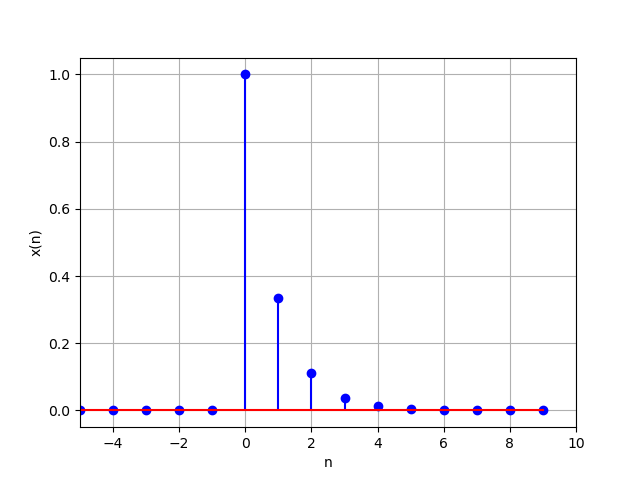
\includegraphics[width = \columnwidth]{2021/BT/20/figs/x_plt.png}
    \caption{Plot of $x(n)$ vs $n$}
    \label{fig:1_gate.21.bt.20}
\end{figure}
\begin{figure}[!h]
    \centering
    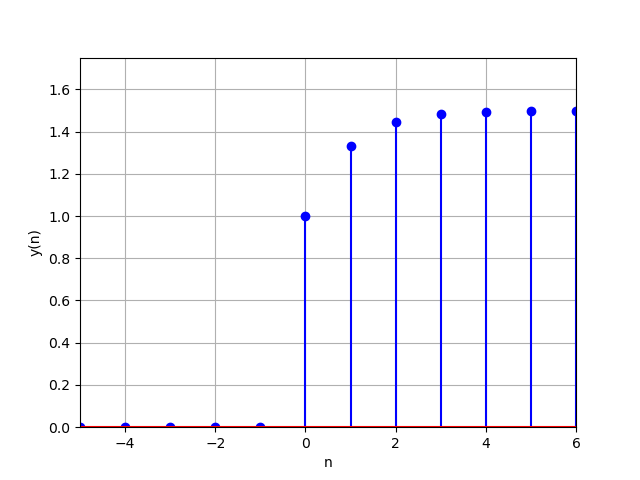
\includegraphics[width = \columnwidth]{2021/BT/20/figs/y_plt.png}
    \caption{Plot of $y(n)$ vs $n$}
    \label{fig:2_gate.21.bt.20}
\end{figure}
%\end{document}

